\hspace{24pt}

This paper attempts to improve the zh-ja NMT system by utilizing the phonetic information hidden in the sentences. Section~\ref{sec:tokenization} explains which tokenization methods we use to deconstruct sentences. Section~\ref{sec:phonetic_data} explains which phonetic extraction methods we use to transform plain sentences into phonetic encodings. Section~\ref{sec:embedding} shows how we use Word2Vec as our algorithm to build and combine semantic and phonetic embeddings. Section~\ref{sec:corpus_filtering} shows how we process data from the corpus to eliminate as much noise and reduce the size of the corpus as possible. Section~\ref{sec:nmt_model} explains the details of two NMT models, which are the Attention-based GRU encoder-decoder Model and Transformer. Section~\ref{sec:embedding_analysis} describes the methods we use to analyze the difference between semantic embeddings and joint semantic-phonetic embeddings.

\section{Tokenization} \label{sec:tokenization}

This paper will examine the effectiveness of phonetic information under different tokenization methods. We use the \textit{tokenizers} \footnote{https://github.com/huggingface/tokenizers} library from the \textit{huggingface} team as our main framework for tokenization. SentencePiece \footnote{https://github.com/google/sentencepiece}, Jieba, and Janome can be implemented as pre-tokenizers in Huggingface Tokenizers.

\subsection{Huggingface Tokenizers} \label{sec:tokenizers}

Huggingface Tokenizers has 5 components that allow users to customize their tokenization methods. These five components are normalizers, pre-tokenizers, models, post-processors, and decoders. Normalizers process an input string such as lower cases or remove spaces and symbols to make it normalized. Pre-tokenizers split an input string according to a set of rules, and pre-tokenizers are where we apply SentencePiece, Jieba, and Janome. Models are responsible for converting text into ids by using the rules learned in the corpus (e.g., WordPiece, BPE, Unigram). Post-processors help us to insert special tokens into the sentence, such as the start token \textit{[BOS]} and the end token \text{[EOS]} in NMT tasks. Lastly, the job of Decoders is to reverse the ids to the original sentence.

\subsection{Byte-Pair Encoding (BPE)} \label{sec:bpe}

We use BPE as the model for merging Chinese and Japanese tokens. BPE builds a dictionary of all the words in the corpus and merges the most frequent words to generate new tokens until the maximum number of our dictionary is reached. We demonstrate the basic flow of BPE applied to Chinese through Table \ref{tab:bpe1} and \ref{tab:bpe2}.  

\vspace{0.5cm}
\begin{CJK}{UTF8}{gbsn}
\begin{table}[h]
    \centering
    \begin{tabularx}{.9\textwidth}{sbb}\toprule
        Frequency & Vocabulary & Dictionary \\
        5 & 区\enspace\_ & \_,\enspace区,\enspace地,\enspace经,\enspace济 \\
        7 & 地\enspace区\enspace\_& \\
        3 & 地\enspace区\enspace经\enspace济\enspace\_ & \\
        6 & 经\enspace济\enspace\_ & \\
        \bottomrule
    \end{tabularx}
    \caption{A simple dataset for demonstrating BPE tokenization}
    \label{tab:bpe1}
\end{table}
\end{CJK}

Words are first tokenized by pre-tokenizers and loaded into the BPE vocabulary, with the underscore (\_) representing the end of the words.

\vspace{0.5cm}
\begin{CJK}{UTF8}{gbsn}
    \begin{table}[h]
        \centering
        \begin{tabularx}{.9\textwidth}{ssb}\toprule
            Total Frequency & Merge & New Dictionary \\
            12 & (区,\enspace\_) & \_,\enspace区,\enspace地,\enspace经,\enspace济,\enspace区\_ \\
            9  & (济,\enspace\_) & \_,\enspace区,\enspace地,\enspace经,\enspace济,\enspace区\_,\enspace济\_ \\
            9  & (经,\enspace济\_) & \_,\enspace区,\enspace地,\enspace经,\enspace济,\enspace区\_,\enspace济\_,\enspace经济\_ \\
            7  & (地,\enspace区\_) & \_,\enspace区,\enspace地,\enspace经,\enspace济,\enspace区\_,\enspace济\_,\enspace经济\_,\enspace地区\_ \\
            \bottomrule
        \end{tabularx}
        \caption{The process of merging tokens in BPE tokenization}
        \label{tab:bpe2}
    \end{table}
\end{CJK}

\begin{CJK}{UTF8}{gbsn}
The merge begins with 区 and \_, which appear most frequently in the vocabulary. After merging, 区\_ will be added to the final dictionary and replaces (区\enspace\_) in the vocabulary. This process continues until the final dictionary reaches its maximum size.
\end{CJK}

\subsection{SentencePiece} \label{sec:sentencepiece}

SentencePiece treats all text in the same Unicode format. It will escape the white space with a meta symbol `\_' (U+2581). Therefore, the sentences in Chinese, Japanese, and English are considered to be in the same format, which achieving language independence. 

SentencePiece is a purely data-driven method, which means it relies on the corpus to learn the tokenization. It is simple to implement SentencePiece in Huggingface Tokenizers. First, Normalization Form Compatibility Composition (NFKC) normalizes the sentence, for example, by converting a symbol or text in the full-width form to a normalized form. Second, Metaspace pre-tokenizer splits the sentence by white space and converts the white space into the `\_' symbol. Last, BPE with dropout is applied to train with the corpus file. The dropout method will improve the robustness and accuracy.

\vspace{0.5cm}

\begin{python}
from tokenizers.normalizers import NFKC
from tokenizers import Tokenizer, pre_tokenizers, decoders, trainers

tokenizer = Tokenizer(BPE(dropout=dropout, unk_token="[UNK]"))
tokenizer.normalizer = NFKC()
tokenizer.pre_tokenizer = pre_tokenizers.Metaspace(replacement="_", add_prefix_space=True)
tokenizer.decoder = decoders.Metaspace(replacement="_", add_prefix_space=True)

trainer = trainers.BpeTrainer(vocab_size=vocab_size)
tokenizer.train(corpus, trainer=trainer)
\end{python}

\subsection{Jieba} \label{sec:jieba}

Jieba is a famous Chinese tokenization Python library that has more than 26,000 stars on Github currently. Jieba uses a prefix dictionary to store the words and calculates the longest path from the Directed Acyclic Graph (DAG) created by the sentences and dictionary to return the most likely tokenized words. In addition, Jieba uses Hidden Markov Model (HMM) and Viterbi algorithm to tokenized the unknown words in the prefix dictionary. There are four states (B, M, E, S) in the HMM model, which represent the beginning, middle, end, and single (the character can represent a word) of a character. The Viterbi algorithm takes all the words as observation and outputs the states of each character from the input sentence. 

A single line of code \pythoninline{jieba.tokenize(sentence_str)} can obtain the tokenized words from Jieba. We inserted it into Huggingface Tokenizers as a pre-tokenizer and trained the Chinese dictionary using BPE.

\vspace{0.5cm}

\begin{python}
    class JiebaPreTokenizer:
    def jieba_split(self, i: int, normalized_string: NormalizedString) -> List[NormalizedString]:
        splits = []
        for _, start, stop in jieba.tokenize(str(normalized_string)):
            splits.append(normalized_string[start:stop])
        return splits
    
    def pre_tokenize(self, pretok: PreTokenizedString):
         pretok.split(self.jieba_split)
\end{python}

\newpage

\subsection{Janome} \label{sec:janome}

Janome is a Japanese tokenization Python library that currently has 600 stars on Github. It applied the Japanese dictionary of another famous tokenization library, mecab \footnote{https://github.com/taku910/mecab}. For the methodology, Janome used the Minimal Acyclic Subsequential Transducer (MAST) as the internal dictionary data structure and the Viterbi algorithm to calculate the probability of tokenized words.

We inserted the Janome tokenizer as a pre-tokenizer to Huggingface Tokenizers and trained the Japanese dictionary using BPE.

\vspace{0.3cm}

\begin{python}
ja_tokenizer = janome.tokenizer.Tokenizer()

class JanomePreTokenizer:
    def janome_split(self, i: int, normalized_string: NormalizedString) -> List[NormalizedString]:
        splits = []
        i = 0
        for token in ja_tokenizer.tokenize(str(normalized_string).strip(), wakati=True):
            splits.append(normalized_string[i: i+len(token)])
            i += len(token)
        return splits
    
    def pre_tokenize(self, pretok: PreTokenizedString):
        pretok.split(self.janome_split)

\end{python}

\subsection{Comparison of Tokenizers} \label{sec:compare_tokenizers}

A sample of tokenized sentences using three tokenizers is listed in Table~\ref{tab:tokenized_sentences}. Jieba and Janome can tokenize the words more precisely than SentencePiece. The better performance of Jieba and Janome over SentencePiece can be considered to be due to the small size and domain specificity of the corpus.

\vspace{0.4cm}
\begin{CJK}{UTF8}{gbsn}
    \begin{table}[h]
        \centering
        \begin{tabularx}{\textwidth}{lb}\toprule
            Input (Chinese) & 平成15年进行的研究内容如下。\\
            SentencePiece & [\_平成, \_15, \_年, 进行的研究, 内容, 如下, \_。] \\
            Jieba & [平成, 15, 年, 进行, 的, 研究, 内容, 如下, 。] \\\midrule
            Input (Japanese) & 平成15年度に行なった研究内容は次の通りである。 \\
            SentencePiece & [\_平成, \_15, \_年度, に行, なった, 研究, 内容, は次の通りである, \_。] \\
            Janome & [平成, 15, 年度, に, 行なっ, た, 研究, 内容, は, 次, の, 通り, で, ある, 。] \\
            \bottomrule
        \end{tabularx}
        \caption{Tokenized sentences using three tokenizers}
        \label{tab:tokenized_sentences}
    \end{table}
\end{CJK}

\newpage

\section{Phonetic Data Extraction} \label{sec:phonetic_data}

Dragonmapper \footnote{https://github.com/tsroten/dragonmapper} is used to extract information from Chinese sentences. Pykakasi \footnote{https://github.com/miurahr/pykakasi} is used to extract information from Japanese sentences.

\subsection{Dragonmapper} \label{sec:dragonmapper}

Dragonmapper is a Python library that can convert between Chinese characters, Bopomofo, Pinyin, and International Phonetic Alphabet (IPA). When we call \pythoninline{dragonmapper.hanzi.to_pinyin(chinese_str)}, it will convert the Chinese sentence to Bopomofo tokens based on \textit{CC-CEDICT} \footnote{https://cc-cedict.org/wiki/} and \textit{Unihan} \footnote{http://www.unicode.org/charts/unihan.html} database. Table \ref{tab:dragonmapper} shows the result of phonetic extraction in Chinese sentences. The extraction will be applied to the tokenized sentences to achieve better accuracy.

\vspace{0.2cm}

    \begin{table}[h]
        \centering

        \begin{CJK*}{UTF8}{gbsn}
            \begin{tabular}{p{2.3cm}p{12cm}}\toprule
                Input & 数据详细计量对于节能推进的重要性 \\
                Tokenized & [数据, 详细, 计量, 对于, 节能, 推进, 的, 重要性] \\
            \end{tabular}
        \end{CJK*}
        
        \begin{CJK}{UTF8}{bsmi}
        \begin{tabular}{p{2.3cm}p{12cm}}
            Extracted & [ㄕㄨˋ ㄐㄩˋ,\enspace
            ㄒㄧㄤˊ ㄒㄧˋ,\enspaceㄐㄧˋ ㄌㄧㄤˋ,\enspaceㄉㄨㄟˋ ㄩˊ,\enspaceㄐㄧㄝˊ ㄋㄥˊ,\enspaceㄊㄨㄟ ㄐㄧㄣˋ,\enspaceㄉㄜ˙,\enspaceㄓㄨㄥˋ ㄧㄠˋ ㄒㄧㄥˋ]
        \end{tabular}
        \end{CJK}

        \begin{CJK*}{UTF8}{gbsn}
            \begin{tabular}{p{2.3cm}p{12cm}}\toprule
                Input & 分析项目是1997-2001年是砷、镍、锰、铬、铍 \\
                Tokenized & [分析, 项目, 在, 1997, -, 2001, 年, 是, 砷, 、, 镍, 、, 锰, 、, 铬, 、, 铍] \\
            \end{tabular}
        \end{CJK*}
        
        \begin{CJK}{UTF8}{bsmi}
        \begin{tabular}{p{2.3cm}p{12cm}}
            Extracted & [ㄈㄣ ㄒㄧ,\enspaceㄒㄧㄤˋ ㄇㄨˋ,\enspaceㄗㄞˋ,\enspace1997,\enspace-,\enspace2001,\enspaceㄋㄧㄢˊ,\enspaceㄕˋ,\enspaceㄕㄣ,\enspace、,\enspaceㄋㄧㄝˋ,\enspace、,\enspaceㄇㄥˇ,\enspace、,\enspaceㄍㄜˋ,\enspace、,\enspaceㄆㄧ]
        \end{tabular}
        \end{CJK}

        \begin{CJK*}{UTF8}{gbsn}
            \begin{tabular}{p{2.3cm}p{12cm}}\toprule
                Heteronym Test & 长大很快乐,音乐很长久 \\
                Tokenized & [长大, 很, 快乐, ,, 音乐, 很, 长久] \\
            \end{tabular}
        \end{CJK*}
        
        \begin{CJK}{UTF8}{bsmi}
        \begin{tabular}{p{2.3cm}p{12cm}}
            Extracted & ['ㄓㄤˇ ㄉㄚˋ,\enspaceㄏㄣˇ,\enspaceㄎㄨㄞˋ ㄌㄜˋ,\enspace,,\enspaceㄧㄣ ㄩㄝˋ,\enspaceㄏㄣˇ,\enspaceㄔㄤˊ ㄐㄧㄡˇ] \\\bottomrule
        \end{tabular}
        \end{CJK}

        \caption{Chinese Phonetic Extraction using Dragonmapper library}
        \label{tab:dragonmapper}
    \end{table}

\subsection{Pykakasi} \label{sec:pykakasi}

Pykakasi is a Python library that implements algorithms in \textit{kakasi} \footnote{http://kakasi.namazu.org/index.html.en} library. It is able to convert Kanji characters to Hiragana, Katakana, and Romaji through the SKK Japanese dictionary \footnote{https://github.com/skk-dev/dict} and UniDic \footnote{https://unidic.ninjal.ac.jp/}. Table \ref{tab:pykakasi} shows the result of phonetic extraction in Japanese tokenized sentences. 

\vspace{0.2cm}

\begin{CJK}{UTF8}{long}
    \begin{table}[h]
        \centering
            \begin{tabular}{p{2.3cm}p{12cm}}\toprule
                Input & 技術以外にも,政策、法律、社会的側面の課題がある \\
                Tokenized & [技術, 以外, に, も, ,, 政策, 、, 法律, 、, 社会, 的, 側面, の, 課題, が, ある] \\
                Extracted & [ぎじゅつ,\enspaceいがい,\enspaceに,\enspaceも,\enspace,,\enspaceせいさく,\enspace、,\enspaceほうりつ,\enspace、,\enspaceしゃかい,\enspaceてき,\enspaceそくめん,\enspaceの,\enspaceかだい,\enspaceが,\enspaceある] \\\midrule

                Input & 冠状動脈レントゲンでTIMI血流3級が示された \\
                Tokenized & [冠状, 動脈, レントゲン, で, TI, MI, 血流, 3, 級, が, 示さ, れ, た] \\
                Extracted & [かんじょう,\enspaceどうみゃく,\enspaceれんとげん,\enspaceで,\enspace TI,\enspace MI,\enspaceけつりゅう,\enspace3,\enspaceきゅう,\enspaceが,\enspaceしめさ,\enspaceれ,\enspaceた]\\\midrule

                Heteronym Test & 一生,芝生で生ビールを飲む \\
                Tokenized & [一生, ,, 芝生, で, 生, ビール, を, 飲む] \\
                Extracted & [いっしょう, ,, しばふ, で, なま, びーる, を, のむ] \\\bottomrule

            \end{tabular}
        \caption{Japanese Phonetic Extraction using Pykakasi library}
        \label{tab:pykakasi}
    \end{table}
\end{CJK}

% https://bamtercelboo.github.io/2018/03/24/word2vec/
\section{Embedding} \label{sec:embedding}

This paper uses Word2Vec as an embedding framework. Embedding is a distribution representation of words. Compared to using sparse vectors such as one-hot representations to represent words, embedding can represent words as high-dimensional vectors of real numbers. These vectors can be used to obtain similarity between words by computing distances such as cosine similarity. 

First, We will explore the details of Word2Vec. Second, we explain how to train a general word embedding with semantics from a corpus. Third, we examine how to manipulate the phonetic information to build a phonetic embedding. Finally, we combine two embeddings to a joint embedding which can have both semantic and phonetic information.

\subsection{Word2Vec} \label{sec:word2vec}

Word2Vec has two classic papers. The first one \cite{mikolov2013efficient} contributes two approaches to constructing an embedding, namely CBOW and Skip-gram. The second one \cite{mikolov2013distributed} contributes the improved methods of embedding construction, such as Hierarchical Softmax and Negative Sampling. We will use Skip-gram and Negative Sampling to generate word embeddings in this paper.

Skip-gram model uses a neural network with hidden layers to predict the likelihood of context words $w_{t-2}, w_{t-1}, w_{t+1}, w_{t+2}$ of an input word $w_t$. The input word and context words will be paired, such as $(w_t, w_{t-2}), (w_t, w_{t-1})$ to perform supervised training. The model can be expressed as the following equation, where $\theta$ represents hidden states of the input word $w_\text{center}$, and $w_1, w_2, \cdots, w_C$ represents the context words of $w_\text{center}$ within the window size $C$. 

% The goal is to maximize the likelihood of the occurrence of context words for each word $w$ in the corpus by updating $\theta$ iteratively.

\begin{equation}
\underset{\theta}{\operatorname{argmax}} \, p\left(w_{1}, w_{2}, \ldots, w_{C} \mid w_{\text {center}} ; \theta\right)
\end{equation}

Skip-gram uses the softmax model for context word classification. $h$ is the hidden layer word vector for the input word $w_\text{center}$ from the input embedding matrix, and $W_{\text {output}}$ is a row vector for a context word from the output embedding matrix. $W_{\text {output}_{(c)}}$ corresponds to the row vector of the context word in (input, context) pair, while $W_{\text {output}_{(i)}}$ corresponds to the row vector of each word in the corpus of size $V$.

\begin{equation}
    p\left(w_{\text {context}} \mid w_{\text {center}}\right)=\frac{\exp \left(W_{\text {output}_{{(c)}}} \cdot h\right)}{\sum_{i=1}^{V} \exp \left(W_{\text {output}_{(i)}} \cdot h\right)} \in \mathbb{R}^{1}
\end{equation}

The goal is to obtain the conditional probability distribution of each unique word observed in the corpus given an input word.

\begin{equation}
    \left[\begin{array}{c}
    p\left(w_{1} \mid w_{\text {input}}\right) \\
    p\left(w_{2} \mid w_{\text {input}}\right) \\
    p\left(w_{3} \mid w_{\text {input}}\right) \\
    \vdots \\
    p\left(w_{V} \mid w_{\text {input}}\right)
    \end{array}\right]=\frac{\exp \left(W_{\text {output }_{(c)}} \cdot h\right)}{\sum_{i=1}^{V} \exp \left(W_{\text {output }_{(i)}} \cdot h\right)} \in \mathbb{R}^{V}
\end{equation}

In machine learning, it is a convention to minimize the loss function. The log is added to the equation to simplify and accelerate the calculation, and the formula is rewritten as minimizing a negative log-likelihood instead of maximizing a positive log-likelihood.

\begin{align}
J\left(\theta ; w^{(t)}\right)&=-\log \prod_{c=1}^{C} \frac{\exp \left(W_{\text {output }_{(c)}} \cdot h\right)}{\sum_{i=1}^{V} \exp \left(W_{\text {output }_{(i)}} \cdot h\right)} \\
&=-\sum_{c=1}^{C} \log \frac{\exp \left(W_{\text {output }_{(c)}} \cdot h\right)}{\sum_{i=1}^{V} \exp \left(W_{\text {output }_{(i)}} \cdot h\right)} \\
&=-\sum_{c=1}^{C}\left(W_{\text {output }_{(c)}} \cdot h\right)+C \cdot \log \sum_{i=1}^{V} \exp \left(W_{\text {output }_{(i)}} \cdot h\right)
\end{align}

Figure~\ref{fig:skip-gram} shows the Skip-gram model. we will learn word embedding vectors of size $N$ given the vocabulary size $V$. The model uses one input word at a time for learning to predict one context word (output).

\begin{figure}[h]
	\centering
	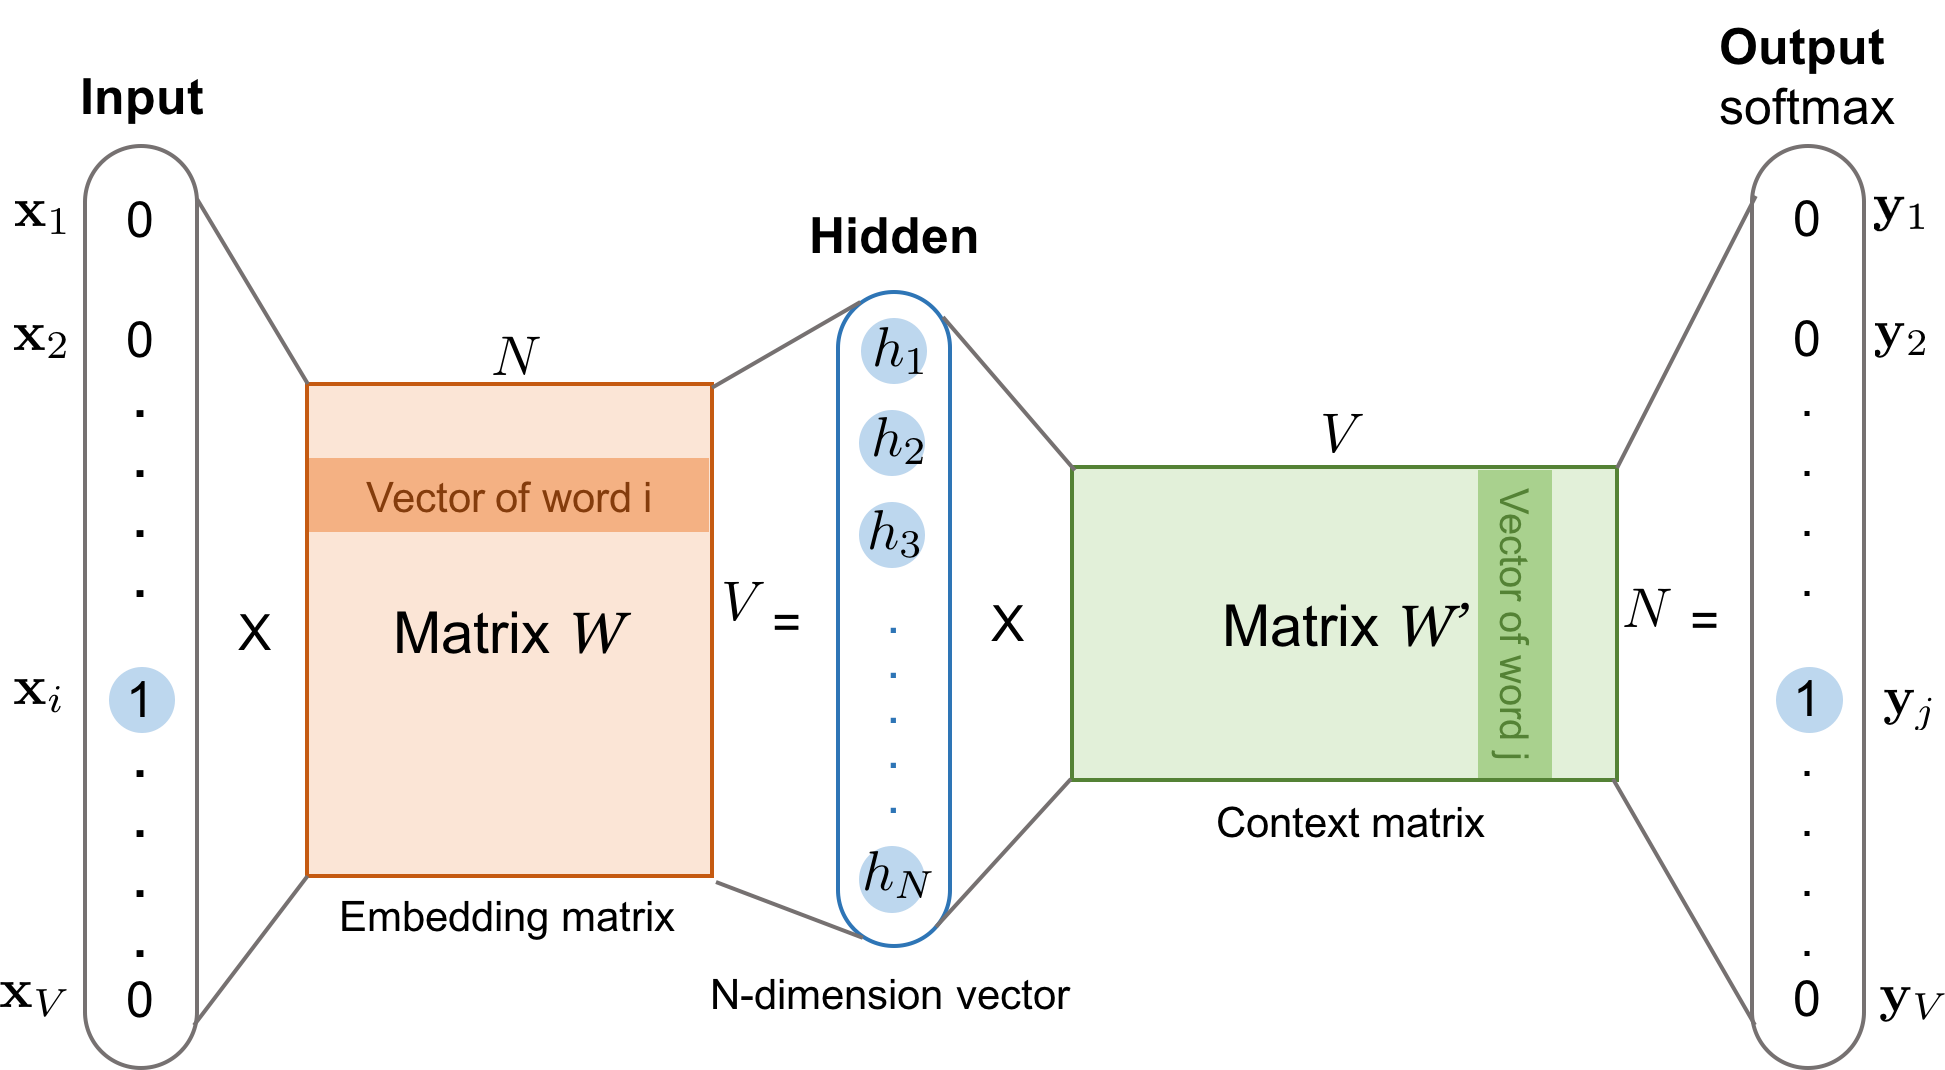
\includegraphics[scale=0.4]{../images/skip-gram.png}
    \caption[The Skip-gram Model]{The Skip-gram Model\protect\footnotemark}
	\label{fig:skip-gram}
\end{figure}

\footnotetext{Source: https://lilianweng.github.io/lil-log/2017/10/15/learning-word-embedding.html}

Since the softmax model requires a lot of computational space and time, we also use negative sampling with the Skip-gram model. Negative sampling will convert the multi-classification problem that the model is designed to solve into a binary-classification problem. First, the method will randomly select $K$ negative samples from the corpus that are irrelevant to the input word. $K$ is a hyper-parameter, usually between 5 and 20. The model will update $(K+1)\times N$ parameters using the sigmoid function, where $N$ is the dimension of the hidden layer $h$, and $+1$ accounts for the positive sample.

The probability that a word ($c$) appears within the context of the input word ($w$) can be defined as the following formula. The goal is to determine whether $c$ is in the context window of $w$ ($D=1$) or not ($D=0$) based on the input-context pairs $(w, c)$.

\begin{equation}
p(D=1 \mid w, c ; \theta)=\frac{1}{1+\exp \left(-\bar{c}_{\text {output }_{(j)}} \cdot w\right)} \in \mathbb{R}^{1}
\end{equation}

\subsection{Semantic Embedding}

We use gensim to implement Skip-gram with negative sampling from Word2Vec. We put the tokenized sentences generated by different tokenizers into gensim to train the general word embedding with semantics. The following are the main settings of the parameters: \textit{max\_vocab\_size} is 32000, \textit{vector\_size} is 300, \textit{epoch\_number} is 13, \textit{window\_size} is 5, the number of negative samples is 5, ignoring the words with total frequency lower than 5.

Some words may not be trained in the model, such as special tokens and low-frequency words. Therefore, the size of the trained embedding matrix and the tokenizer vocabulary is not identical, resulting in different coverage (Table~\ref{tab:semantic_coverage}). We calculate the mean and standard deviation of the whole embedding and randomly assign the empty word vectors using the normal distribution.

\vspace{0.5cm}
\begin{table}[h]
    \centering
    \begin{tabularx}{.9\textwidth}{ssss}\toprule
        Language & SentencePiece & Jieba & Janome \\\midrule
        Chinese & 95\% (30368/32000) & 93\% (29613/32000) & - \\
        Japanese & 97\% (30940/32000) & - & 93\% (29801/32000) \\
        \bottomrule
    \end{tabularx}
    \caption{The coverage of semantic embedding in vocabulary}
    \label{tab:semantic_coverage}
\end{table}

\subsection{Phonetic Embedding} \label{sec:phonetic_embedding}

The training method for phonetic embedding is mostly the same as semantic embedding. First, we convert tokenized sentences into phonetic encodings using the phonetic extraction techniques described in Section~\ref{sec:phonetic_data}. Second, we adopt the same training methods and parameters from semantic embedding. And last, we share the same vector of characters or words with the same pronunciation or spelling in the embedding matrix. Therefore, the coverage (Table~\ref{tab:phonetic_coverage}) will be even higher than the semantic embedding. The empty vectors are also randomly assigned using the normal distribution with mean and standard deviation from the whole embedding. 

\vspace{0.5cm}
\begin{table}[h]
    \centering
    \begin{tabularx}{.9\textwidth}{ssss}\toprule
        Language & SentencePiece & Jieba & Janome \\\midrule
        Chinese & 99\% (31753/32000) & 97\% (31068/32000) & - \\
        Japanese & 99\% (31698/32000) & - & 96\% (30809/32000) \\
        \bottomrule
    \end{tabularx}
    \caption{The coverage of phonetic embedding in vocabulary}
    \label{tab:phonetic_coverage}
\end{table}

\subsection{Joint Embedding} \label{sec:joint_embedding}

Several ways have been proposed to combine multiple embeddings, such as concatenation, training and blending separate embedding using the same model, and meta-embedding. Meta-embedding is a very vague term, but the core idea is to accept any kind of pre-trained embedding and fuse them into one (meta) embedding. Many studies on meta-embedding have been proposed \cite{kiela-etal-2018-dynamic, yin2015learning, muromagi2017linear}. The methods of meta-embedding can range from very complicated to very straightforward. This paper uses a simple averaging method \cite{coates-bollegala-2018-frustratingly} to merge semantic and phonetic embedding.

\section{Corpus Filtering} \label{sec:corpus_filtering}

% 為了是減少噪音以及 nmt 訓練時的資源負擔

% 用了哪些方法

\subsection{Pre-filtering rules}

% 列出並解釋每個方法

\subsection{Scoring functions}

% align 打分數

% 最終剩下多少句子

\section{NMT Model} \label{sec:nmt_model}

% 我們使用兩種模型來訓練 NMT 任務。分別是基於某論文提的。以及某某論文提起。模型的參數在哪裡提,模型的評分在哪裡提。模型的結果在哪裡提。關於翻譯的句子 case study 會在哪裡提。

\subsection{Attention-based GRU encoder-decoder Model} \label{sec:rnn}

% 先講所有架構。

% 分別講每個架構。每個架構的圖,公式。

\subsection{Transformer} \label{sec:transformer}

% 先講所有架構。

% 分別講每個架構。每個架構的圖,公式。

% https://bamtercelboo.github.io/2018/05/12/embedding_evaluation/
\section{Embedding Analysis} \label{sec:embedding_analysis}

% 我們使用四種方法驗證有效性。希望XX能保留效果,希望能加強 4。我們用 gensim 來實作這四個驗證。驗證結果會在 discussion 討論。

\subsection{Analogy Reasoning} \label{sec:analogy}

% 講解這個東西在幹嘛的。怎麼算。怎麼用 gensim 跑。

\subsection{Outlier Detection} \label{sec:outlier}

% 講解這個東西在幹嘛的。怎麼算。怎麼用 gensim 跑。

\subsection{Word Similarity} \label{sec:similarity}

% 講解這個東西在幹嘛的。怎麼算。怎麼用 gensim 跑。

\subsection{Homonym and Heteronym} \label{sec:homonym_heteronym}

% 講解這個東西在幹嘛的。怎麼算。怎麼用 gensim 跑。
